%-----------------------------------------------------------------------------
%
%               Template for sigplanconf LaTeX Class
%
% Name:         sigplanconf-template.tex
%
% Purpose:      A template for sigplanconf.cls, which is a LaTeX 2e class
%               file for SIGPLAN conference proceedings.
%
% Guide:        Refer to "Author's Guide to the ACM SIGPLAN Class,"
%               sigplanconf-guide.pdf
%
% Author:       Paul C. Anagnostopoulos
%               Windfall Software
%               978 371-2316
%               paul@windfall.com
%
% Created:      15 February 2005
%
%-----------------------------------------------------------------------------


\documentclass[10pt]{sigplanconf}

% The following \documentclass options may be useful:

% preprint      Remove this option only once the paper is in final form.
% 10pt          To set in 10-point type instead of 9-point.
% 11pt          To set in 11-point type instead of 9-point.
% numbers       To obtain numeric citation style instead of author/year.

\usepackage{amsmath}
\usepackage{booktabs}
\usepackage{amsfonts}
\usepackage{listings}
\usepackage{graphicx}
%\usepackage{breqn}
\usepackage{rotating}
\usepackage{pbox}
\usepackage{subfig}
\usepackage{hyperref}
\usepackage{backnaur}
\usepackage{algorithm2e}
\usepackage{listings}
\usepackage{array}
\usepackage{url}

\newcommand{\cL}{{\cal L}}

\begin{document}

\special{papersize=8.5in,11in}
\setlength{\pdfpageheight}{\paperheight}
\setlength{\pdfpagewidth}{\paperwidth}

%\CopyrightYear{2017} 
%\setcopyright{rightsretained} 
%\conferenceinfo{PPoPP '17}{February 04-08, 2017, Austin, TX, USA} 
%\isbn{978-1-4503-4493-7/17/02}
%\doi{http://dx.doi.org/10.1145/3018743.3019027}

%\conferenceinfo{PPoPP '17}{February 04-08, 2017, Austin, TX, USA} 
%\copyrightyear{2017}
%\copyrightdata{978-1-4503-4493-7/17/02}
%\copyrightdoi{3018743.3019027}

%\permissiontopublish
%\conferenceinfo{PPoPP~'17}{Feb. 4--8, 2017, Austin, Texas, USA.} 
%\copyrightyear{2017} 
%\copyrightdata{978-1-4503-4493-7/17/02} 
%\doi{3018743.3019027} 

% Uncomment the publication rights you want to use.
%\publicationrights{transferred}
%\publicationrights{licensed}     % this is the default
%\publicationrights{author-pays}

%\titlebanner{banner above paper title}        % These are ignored unless
%\preprintfooter{short description of paper}   % 'preprint' option specified.

\title{Semantic-aware anomaly detection in real world parking data}
%\subtitle{Subtitle Text, if any}

\authorinfo{Arnamoy Bhattacharyya, Weihan Wang, Cristine Tang, Cristiana Amza}


\maketitle

\begin{abstract}
In this work, we introduce and experimentally evaluate a novel approach for anomaly detection in smart car parking applications.  We attach semantics to the raw parking data collected from sensors of parking lots to detect anomalous patterns in them.  Attaching semantics on top of raw data helps reduce the processing time and also provides the error checker a distinct context to look into potential problems.
\end{abstract}

%\section{Goal}
%
%The goal of the first step in the semi-automation of the data checking process will be targeted towards the external benchmark checking.  The external benchmark checking consists of the following test cases currently:
%
%\begin{itemize}
%\item Monthly Revenue Check
%\item Daily Revenue Check for the weekdays
%\item Daily Revenue Check 2 for the weekdays
%\item Revenue Check for the weekends
%\item Entries per day
%\item Exits per day
%\item Manual Count per day
%\end{itemize}
%
%The workflow design for semi-automating the above mentioned checks is shown in Figure~\ref{fig:workflow}.  Basically, the AM will input the values collected from the client side in a webpage (the front end).  Then the webpage goes to the back-end server and matched the entered values with the values stored in the databases of Smarking Inc. For all the mismatches found, the result is shown back to the AM. 
%
%\begin{figure}[h]
%\centering
%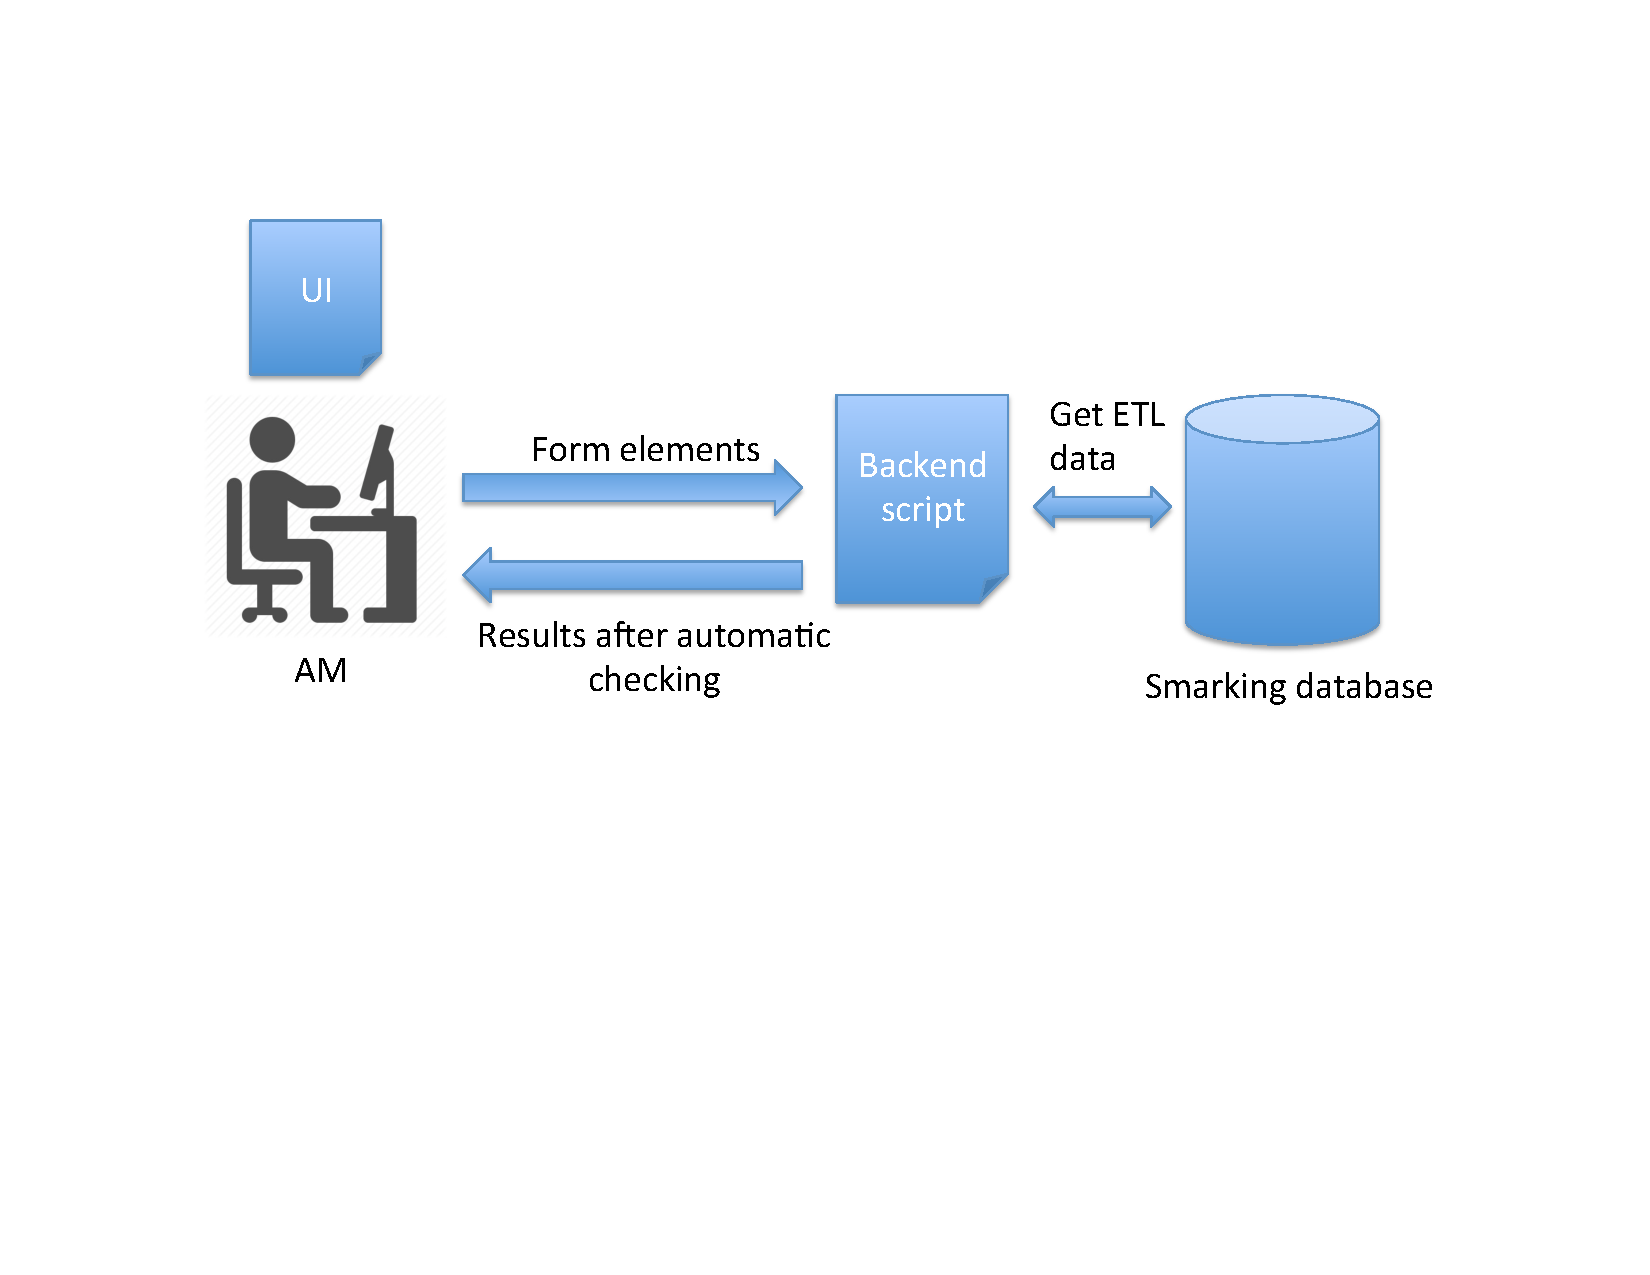
\includegraphics[width=8.3cm]{./figures/workflow.pdf}
%\caption{The workflow of the semi-automated checking.}
%\label{fig:workflow}
%\end{figure}
%
%Figure~\ref{fig:frontend} shows the design of a basic UI for the front end.  The different client side values are added by the AM in the designated text boxes.  Also the date range for that data is given.  The dynamic web page lets the AM add new data ranges for the same garage or for new garages.  For example figure~\ref{fig:frontend} shows two different date ranges for the garage ID and one data range for the garage ID .
%
%Once the data entry is over, the AM presses the  ``check garages'' button.  The entered values goes to the backend script for doing the comparison and the result is shown in Figure~\ref{fig:result}.  Here the garage ID 564765 has two mismatches and garage ID 654786 has one mismatch.
%
%\begin{figure}[h]
%\centering
%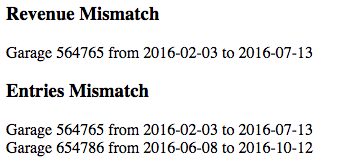
\includegraphics[width=8cm]{./figures/second}
%\caption{The response from the back end as shown to the AM.}
%\label{fig:result}
%\end{figure}
%
%\begin{figure*}[h]
%\centering
%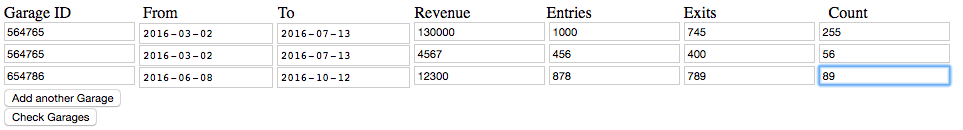
\includegraphics[width=19cm]{./figures/first}
%\caption{Front end presented to the AM.}
%\label{fig:frontend}
%\end{figure*}
\section{Introduction}
TODO
\section{A Semantic Aware Anomaly Detection Approach}

The data we are analyzing has different car occupancy metrics for parking data collected from the parking lots at various locations.  There are two types of car occupancy: contract based cars and transient parkers.

The data we have is for $n$ garages, collected over $m$ hours.

\begin{equation}
contacts = \left \{   con_1, con_2, \ldots , con_n \right \}
\end{equation}

\begin{equation}
transients =   \left \{  tran_1, tran_2, \ldots , tran_n \right \}
\end{equation}

Parking data for each garage $i$ ($i \in n$) has the data for $m$ months and has the following form:

\begin{equation}
con_i =   \left \{  mon_1, mon_2, \ldots , mon_m \right \}
\end{equation}

\begin{equation}
tran_i =   \left \{  mon_1, mon_2, \ldots , mon_m \right \}
\end{equation}

Each set of monthly parking data $mon_{j}^{i}$ ($i \in n , j \in m$) has $d$ sets of data points, depending on the number of days that month has.  The form for monthly data is:

\begin{equation}
mon_{j}^{i} =   \left \{  day_1, day_2, \ldots , day_d \right \}
\end{equation}

Finally, each set $day_k$ ($k \in d$) has 24 data points, one for each hour of the day.

\subsection{Semantics of the parking data}

To provide a faster analysis of the huge amount of parking data and to provide meaningful feedback to the data checker after the automatic anomaly detection, we attach semantics on top of the raw time-series parking data.  These \textit{modified signals}, with the attached semantics on top are then fed to our anomaly detection methods to find abnormal patterns in them.  We define the following \textit{modified signals} that we derive from the raw parking data:

\begin{enumerate}
\item \textbf{Monthly Peak Occupancy}:  The value of a monthly peak occupancy signal $mon_{pk}$ for a garage $garage_i$ for $m$ months is given by the following equation:

\begin{multline}
\left \{ mon_{pk} \left ( m \right )\right \} =   ( \max\left \{ mon_{1}^{i} \right \}, \max\left \{ mon_{2}^{i} \right \}, \\ 
 \ldots , \max\left \{ mon_{m}^{i} \right \}   ) 
\end{multline}

We further divide the $mon_{pk}$ signal into two finer semantics: contracts ($mon_{pk_{con}}$) and transients($mon_{pk_{tran}}$).  The number of data points in each signal $mon_{pk_{con}}$ and $mon_{pk_{tran}}$ is the number of months under analysis.  This semantics help us to differentiate two distinct parking behaviour patterns for the two parking types.  

\item \textbf{Daily Peak Occupancy}:  The value of a daily peak occupancy signal $day_{pk}$ for a garage $garage_i$ for $d$ days is given by the following equation:

\begin{multline}
\left \{ day_{pk} \left ( d \right )\right \} =   ( \max\left \{ day_{1}^{i} \right \}, \max\left \{ day_{2}^{i} \right \}, \\
\ldots , \max\left \{ day_{d}^{i} \right \}   ) 
\end{multline}

Where $\left \{day_{d}^{i} \right \}$ is the set of hourly occupancies for the d-th day for garage $i$.  Similar to the monthyl peak occupancy, we have two finer semantics $day_{pk_{con}}$ and $day_{pk_{tran}}$ for contracts and transient type of parking.

\item \textbf{Daily Occupancy}:  The daily occupancy is the signal that is comprised of all the 24 datapoints of that given day.  Then we compose a signal $day \left ( d \right )$ that is a concatenation of all the datapoints of $d$ days.  This signal has $24 \dot d$ datapoints.  We have $day_{con}$ and $mon_{tran}$ for contract based and transient parkings respectively.

\end{enumerate}

\subsection{Types of anomalies}
Once we have identified the above semantics (at different granularity levels), we define two different types of anomalies for each semantics.  They are the following:

\begin{enumerate}
\item \textbf{Zero Anomalies}:  When the data value is `0' at certain places.
\item \textbf{Unusual Anomalies}:  When the data values shows unusual values as compared to the other values we are analyzing.
\end{enumerate}

\subsection{Anomaly detection methods}

We use different methods for detecting anomalies at different semantic granularity level.  First we describe those methods.  Then we describe how we optimize our anomaly detection algorithm accordingly as more anomalies are being detected on the training data.  

\begin{enumerate}
\item \textbf{Zero Anomaly detection}:  We detect if there is any zero present in the signals $mon_{pk_{con}}$, $mon_{pk_{tran}}$, $day_{pk_{con}}$ and $day_{pk_{tran}}$.  Once we have detected the zeros on the mentioned signals, we also detect if there are sequences of zeros in those anomalies.  A sequence of zeros in monthly peak occupancies specify a severe error.  A sequence of zeros in the daily peak anomalies specify an error with medium severity.  We do not raise an alarm for zero anomalies in daily occupancy.

\item \textbf{Unusual Anomaly detection}:  Detecting unusual patterns in data is a non-trivial task.  But attaching semantics on top of the raw data helps greatly in detection and defining anomaly categories.

\begin{itemize}
\item Detecting \textit{Global} anomalies:  We use an well-known statistical technique used in outlier detection for detecting these kind of anomalies.  The method is based on Interquartile Range (IQR).  In descriptive statistics, the interquartile range (IQR), also called the midspread or middle 50\%, or technically H-spread, is a measure of statistical dispersion, being equal to the difference between 75th and 25th percentiles, or between upper and lower quartiles.  Data points that falls beyond $\pm 1.5 \dot IQR$ are generally defined as outliers~\cite{navidi2006statistics}.  But from our experiments, a value of $1.5$ was too restrictive.  So we chose a value of $3$.. Anything beyond $\pm 3 \dot IQR$ is flagged as anomalies by our method.

\begin{figure}[h]
\centering
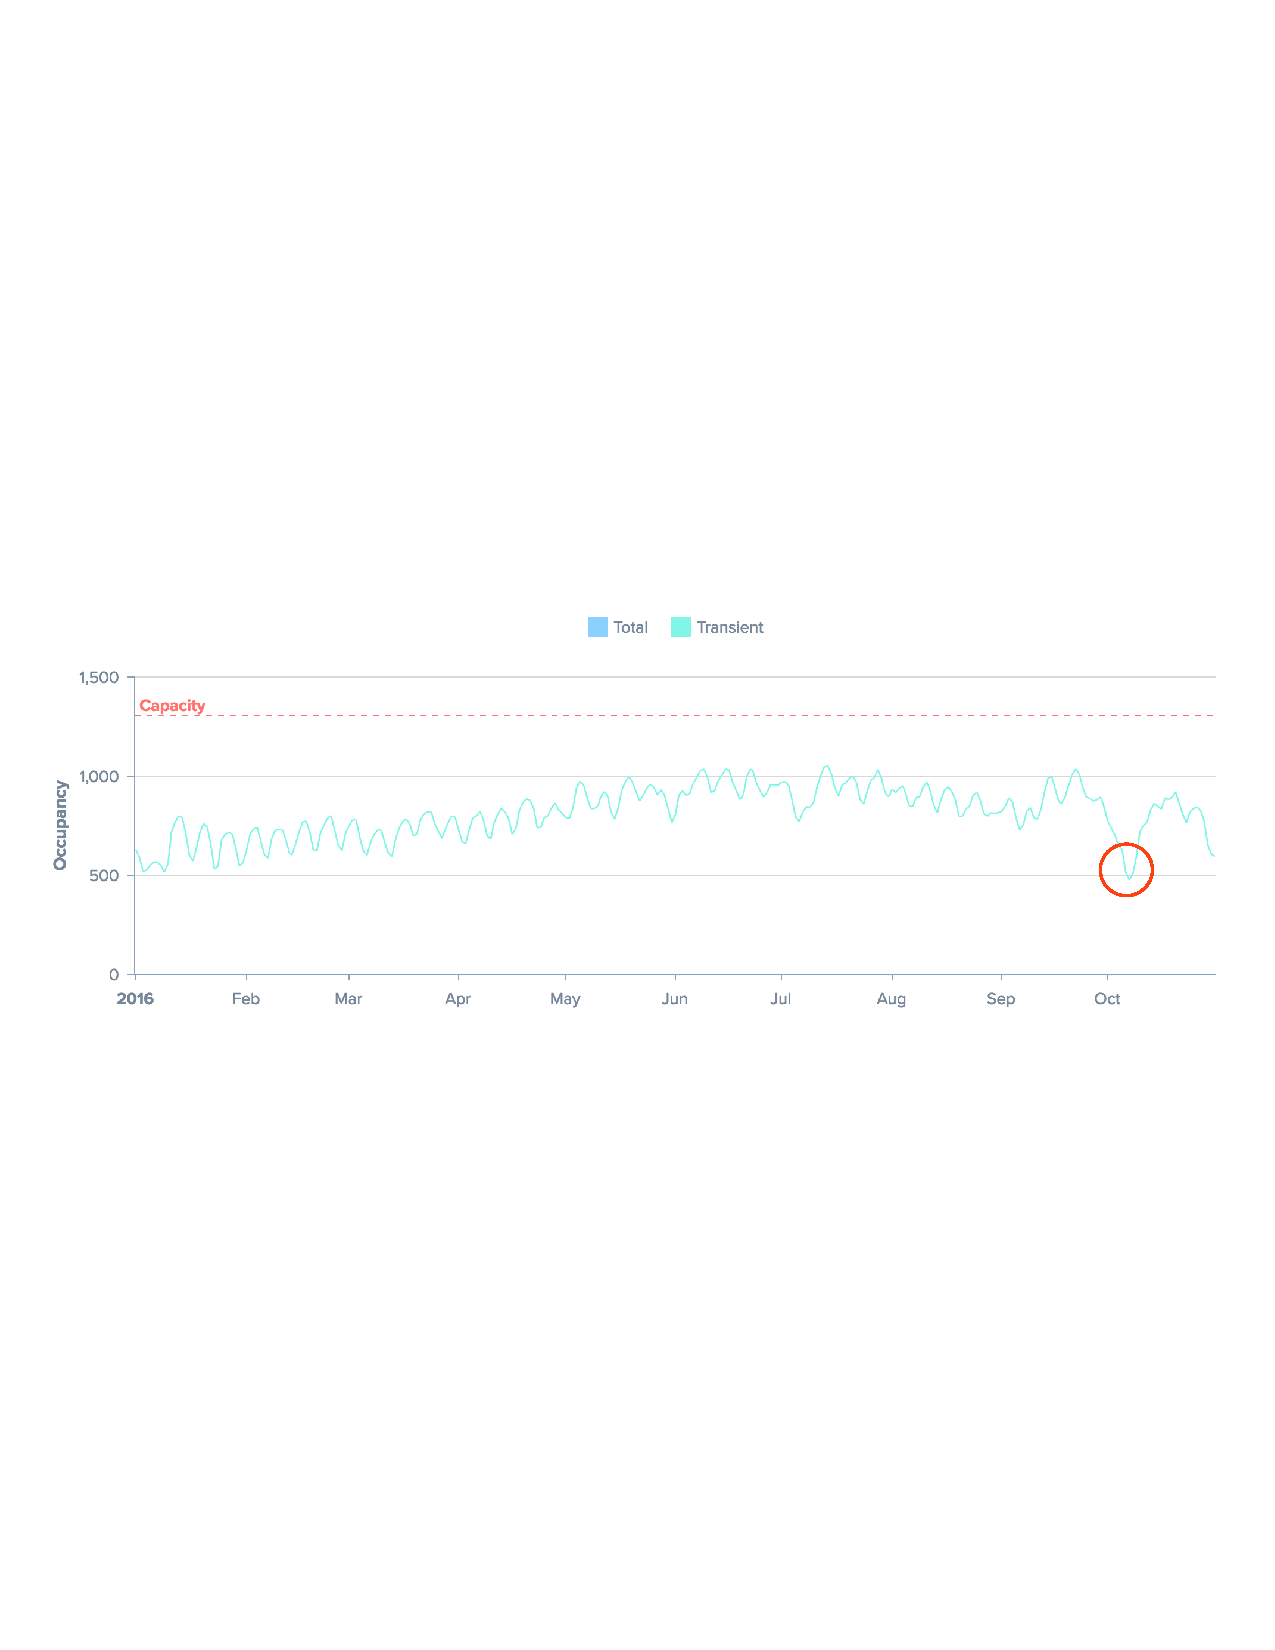
\includegraphics[width=8.4cm]{./figures/local_anomaly.pdf}
\caption{Example of local anomaly.}
\label{fig:local_anomaly}
\end{figure}

\item Detecting \textit{Local} anomalies:  The above method can detect outliers for data where there is not much change over time.  But if there is a trend of increase and decrease in occupancies over time, there can be a few anomalies which are not detected by the above method.  One case is shown in Figure~\ref{fig:local_anomaly}.  Here there was an increasing trend in the daily peak anomalies.  Therefore the anomaly during October (red corcle in figure~\ref{fig:local_anomaly} is not detected by our \textit{global} method as the there are multiple datapoints towards the beginning of the year that will change the nature of the distribution and not flag the anomaly in October.  In these scenarios, we have to look at local trends (months around October) to detect anomalies.  We use a sliding window based approach to detect these \textit{local} anomalies.

We define a window size $w$, calculated by Algorithm~\ref{algo:window}

\begin{algorithm}[h]
\KwIn{data\_size, max\_slides, min\_window}
\KwOut{window\_size}  
num\_slides = 0 \;
window\_size = min\_window \;  
\uIf{data\_size \textless max\_slides}{
    \Return window\_size  \;
    }
 \While{ num\_slides \textless max\_slides } {
 window\_size = data\_size - num\_slides +1 \;
 num\_slides ++ \;
 }
 \Return window\_size  \;
  
\caption{Algorithm to determine the sliding window size for detecting \textit{local} anomalies.}\label{algo:window}
\end{algorithm}

We have a minimum window size min\_window.  The window size window\_size is calculated by a cap on the maximum number of slides, max\_slides.

\item Detecting \textit{minor} anomalies:  Apart from the other two methods, there can still be anomalies that are not typical outliers but they are derivation from usual \textit{patterns} for the metric of consideration.  TODO: Give an example For detecting these anomalies, we use an algorithm called S-H-ESD (ref), or Seasonal Hybrid Extreme Studentized Deviates. This is an extension of a generalized ESD method by adding steps which break down data series into piecewise approximations (a hybrid method) and can account for seasonality in each submodel. Generalized Extreme Studentized Deviates (ESD) is a well established statistical procedure for the detection of outliers where the assumption is that the inliers are normal distributed. The generalized ESD method introduces a procedure for identifying from $1$ to $k$ outliers in a dataset simultaneously thus introducing a robustness for the particular number of outliers present.

The ESD procedure computes statistics $R_1, \dots , R_k$ for $k$ data points as the extreme studentized deviates. The first statistic is the largest deviation from the mean, $R_1 = \underset{i}{\text{max}} \frac{\vert x_i - \bar{x} \vert }{s} , \quad s^2 = \frac{1}{n-1}\sum {(x_i - \bar{x})^2}$  , and the next statistic is calculated on the reduced sample size after removing the sample with the largest deviation, and so on for the subsequent statistics.  Critical values  $\lambda_i$  for each test statistic are determined based on a transformed $t$ distribution for a specified confidence level~\cite{rosner1983percentage}. The decision rule is given as follows: if all of the test statistics are lower than the critical values, then there are no outliers. If any of the test statistics are greater than the critical value, then the largest number of points such that the associated test statistic is greater than the critical value are removed as outliers.

\end{itemize}

\end{enumerate}

\bibliographystyle{abbrv}
\bibliography{references} 

\end{document}
